\section{Lösungsidee}
\begin{wrapfigure}{r}{0.35\textwidth}
	\setlength\intextsep{0pt}
	\centering
	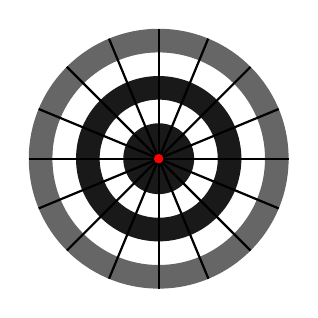
\begin{tikzpicture}[scale=0.3]
	\fill[black!90!white] (0,0) circle [radius=1.5];
	\fill[black!90!white, even odd rule] (0,0) circle[radius=2.5] circle[radius=3.5];
	\fill[black!60!white, even odd rule] (0,0) circle[radius=4.5] circle[radius=5.5];

	\foreach \angle in {0, 22.5, 45, 67.590, 90, 112.5, 135, 157.5, 180, 202.5, 225, 247.5, 270, 292.5, 315, 337.5} 
    	\draw[thick] (0,0) -- (\angle:5.5);

	\fill[red] (0,0) circle[radius=0.2];
\end{tikzpicture}

	\caption{Geraden}
	\label{abb:spidergrafik}
	\vspace{-20pt}
\end{wrapfigure}
Zunächst habe ich den \task{} mit TikZ nachgezeichnet, um den genauen Aufbau durch Nachbau zu verstehen. Die 16 gleichgroßen Kreissegmente sind durch Strahkel getrennt, die im Abstand von \(22,5^{\circ}\) vom Pol (dem Mittelpunkt) aus gezeichnet werden.

Für die Dekodierung steht mir aus dem Kreismittelpunkterkennungsprozess die Liste der Kreismittelpunkte zur Verfügung. Die Kreisdurchmesser entsprechen der Länge der Zusammenhangskomponenten an den Mittelpunktskoordinaten. Mit diesen Informationen kann ich dank bekannter Proportionen eines \task{}s auf die Position des äußeren Ringes, der die Informationen trägt, schließen (siehe Abb. \ref{abb:dims}). Wie in der Lösungsidee zur Kreismittelpunkterkennung festgestellt gilt \(u=\frac{1}{3}d\).

\begin{wrapfigure}{r}{0.25\textwidth}
	\setlength\intextsep{0pt}
	\centering	
	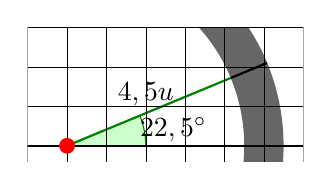
\begin{tikzpicture}[scale=0.5]
	\clip (-1,-0.4) rectangle (6, 3);
	\fill[black!60!white, even odd rule] (0,0) circle[radius=4.5] circle[radius=5.5];

	\foreach \angle in {0, 22.5, 45, 67.590, 90, 112.5, 135, 157.5, 180, 202.5, 225, 247.5, 270, 292.5, 315, 337.5} 
    	\draw[thick] (\angle:4.5) -- (\angle:5.5);

	\filldraw[fill=green!20,draw=green!50!black] (0,0) -- (2,0) arc[start angle=0, end angle=22.5, radius=2];
	\draw[green!50!black, thick] (0,0) -- (22.5:4.5);

	\draw (2, 1.3) node {\(4,5u\)};
	\draw (2.7, 0.4) node {\(22,5^{\circ}\)};

	\draw[very thin] (-6, -6) grid (6, 6);
	\draw[thick] (-6, 0) -- (6, 0);
	\fill[red] (0,0) circle[radius=0.2];
\end{tikzpicture}
	\caption{}
	\label{abb:trigon}
\end{wrapfigure}
Daher kann ich mithilfe von polaren Koordinaten\footnote{\url{https://www.lernhelfer.de/schuelerlexikon/mathematik-abitur/artikel/polarkoordinatensystem}} die Strecken, die die Kreisringe in Segmente einteilen, bestimmen. Jede der Strecken ist Teil eines Strahls, der am Mittelpunkt in einem Vielfachen von \(22,5^{\circ}\) beginnt. Die eigentlichen Strecken, die auf dem äußeren Kreisring liegen, beginnen nach einem Abstand von \(4,5u\) und enden bei \(5,5u\). Die Anfangs- und Endpunkte aller Strecken lauten also:

\begin{displaymath}
A(k \cdot 22,5^{\circ}:4,5u) \hspace{2em} B(k \cdot 22,5^{\circ}:5,5u) \hspace{2em} k = \{\mathbb{N}_0 \hspace{0.3em}|\hspace{0.3em} 0 \le x \le 15\}
\end{displaymath}

Nun können wir aus dieser Koordinatenmenge unter Ausnutzung der Regeln im rechtwinkligen Dreieck (s. Abb \ref{abb:trigon}) die nützlicheren kartesischen Koordinaten bestimmen. Das Koordinatensystem ist in der Einheit \(u\). Bitte beachten Sie, dass sie je nach Programmiersprache oder Taschenrechner zuerst eine Umrechnung der Winkel in Bogenmaß durchführen müssen.

\begin{gather}
k = \{\mathbb{N}_0 \hspace{0.3em}|\hspace{0.3em} 0 \le x \le 15\} \\
\begin{split}
x &= cos(k \cdot 22,5^{\circ}) \cdot 4,5 \\
y &= sin(k \cdot 22,5^{\circ}) \cdot 4,5
\end{split}
\hspace{5em}
\begin{split}
x &= cos(k \cdot 22,5^{\circ}) \cdot 5,5 \\
y &= sin(k \cdot 22,5^{\circ}) \cdot 5,5
\end{split}
\end{gather}

\begin{figure}[!ht]
	\begin{subfigure}[b]{0.5\textwidth}
		\centering	
		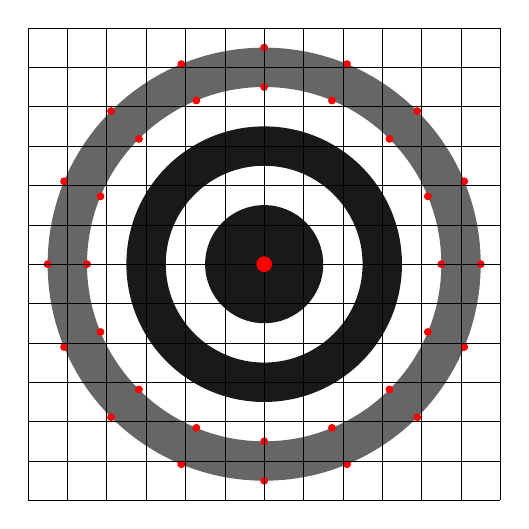
\begin{tikzpicture}[scale=0.5]
	\fill[black!90!white] (0,0) circle [radius=1.5];
	\fill[black!90!white, even odd rule] (0,0) circle[radius=2.5] circle[radius=3.5];
	\fill[black!60!white, even odd rule] (0,0) circle[radius=4.5] circle[radius=5.5];
	
	\fill[red] (4.5,0) circle [radius=0.1]; 
	\fill[red] (5.5,0) circle [radius=0.1]; 
	\fill[red] (4.157457896,1.722075446) circle [radius=0.1]; 
	\fill[red] (5.081337429,2.104758878) circle [radius=0.1]; 
	\fill[red] (3.181980515,3.181980515) circle [radius=0.1]; 
	\fill[red] (3.889087297,3.889087297) circle [radius=0.1]; 
	\fill[red] (1.722075446,4.157457896) circle [radius=0.1]; 
	\fill[red] (2.104758878,5.081337429) circle [radius=0.1]; 
	\fill[red] (2.755455298e-16,4.5) circle [radius=0.1]; 
	\fill[red] (3.367778698e-16,5.5) circle [radius=0.1]; 
	\fill[red] (-1.722075446,4.157457896) circle [radius=0.1]; 
	\fill[red] (-2.104758878,5.081337429) circle [radius=0.1]; 
	\fill[red] (-3.181980515,3.181980515) circle [radius=0.1]; 
	\fill[red] (-3.889087297,3.889087297) circle [radius=0.1]; 
	\fill[red] (-4.157457896,1.722075446) circle [radius=0.1]; 
	\fill[red] (-5.081337429,2.104758878) circle [radius=0.1]; 
	\fill[red] (-4.5,5.510910596e-16) circle [radius=0.1]; 
	\fill[red] (-5.5,6.735557395e-16) circle [radius=0.1]; 
	\fill[red] (-4.157457896,-1.722075446) circle [radius=0.1]; 
	\fill[red] (-5.081337429,-2.104758878) circle [radius=0.1]; 
	\fill[red] (-3.181980515,-3.181980515) circle [radius=0.1]; 
	\fill[red] (-3.889087297,-3.889087297) circle [radius=0.1]; 
	\fill[red] (-1.722075446,-4.157457896) circle [radius=0.1]; 
	\fill[red] (-2.104758878,-5.081337429) circle [radius=0.1]; 
	\fill[red] (-8.266365894e-16,-4.5) circle [radius=0.1]; 
	\fill[red] (-1.010333609e-15,-5.5) circle [radius=0.1]; 
	\fill[red] (1.722075446,-4.157457896) circle [radius=0.1]; 
	\fill[red] (2.104758878,-5.081337429) circle [radius=0.1]; 
	\fill[red] (3.181980515,-3.181980515) circle [radius=0.1]; 
	\fill[red] (3.889087297,-3.889087297) circle [radius=0.1]; 
	\fill[red] (4.157457896,-1.722075446) circle [radius=0.1]; 
	\fill[red] (5.081337429,-2.104758878) circle [radius=0.1]; 

	\draw[very thin] (-6, -6) grid (6, 6);
	\fill[red] (0,0) circle[radius=0.2];
\end{tikzpicture}
		\caption{Einteilenende Punkte}
	\end{subfigure}
	\begin{subfigure}[b]{0.5\textwidth}
		\centering	
		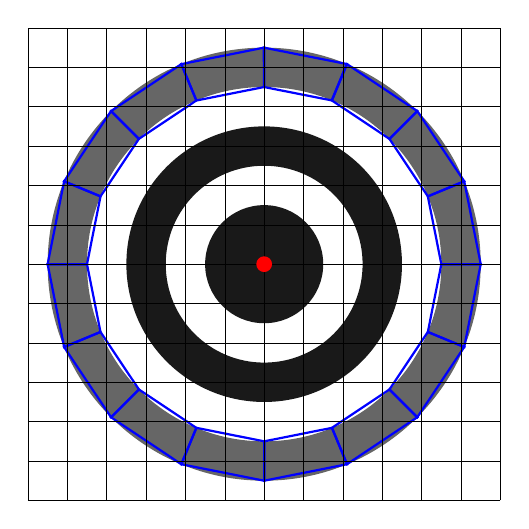
\begin{tikzpicture}[scale=0.5]
	\fill[black!90!white] (0,0) circle [radius=1.5];
	\fill[black!90!white, even odd rule] (0,0) circle[radius=2.5] circle[radius=3.5];
	\fill[black!60!white, even odd rule] (0,0) circle[radius=4.5] circle[radius=5.5];

	\foreach \angle in {0, 22.5, 45, 67.590, 90, 112.5, 135, 157.5, 180, 202.5, 225, 247.5, 270, 292.5, 315, 337.5} 
    	\draw[blue, thick] (\angle:4.5) -- (\angle:5.5) -- (\angle+22.5:5.5) -- (\angle+22.5:4.5) -- cycle;

    	
	\draw[very thin] (-6, -6) grid (6, 6);
	\fill[red] (0,0) circle[radius=0.2];
\end{tikzpicture}
		\caption{Trapeze}
	\end{subfigure}
\end{figure}

Wenn wir nun alle benachbarten Koordinaten verbinden, erhalten wir 16 Trapeze, die fast den Kreissegmenten entsprechen. Da die Abweichung zwischen dem jeweiligen Trapez und dem jeweiligen Kreissegment sehr gering ist, kann aus den Pixeln im Trapez auf die Farbe des Ringsegmentes geschlossen werden. Da das ganze Ringsegment entweder ganz weiß oder ganz schwarz ist, entspricht die vorherrschende Farbe im Trapez der Farbe des Kreissegmentes.
\section{Umsetzung}
\section{Beispiele}